\section{Projektbeispiele}
\label{sec:project-examples}

Dieses Kapitel umfasst einige Ideen für Projekte, die sich gut mit \idename{} umsetzen lassen. Diese Auflistung ist natürlich nicht vollständig, sie umfasst vielmehr jene Projekte die gewissermaßen als "`Proof-of-Concept"' im Rahmen der Entwicklung entstanden sind und sich auch für Lernende eignen könnten.

\subsection{Interaktive Geschichten}
\label{sec:project-cyoa}

Im englischsprachigen Raum hat sich für diese Art von Erzählung der Terminus ``Choose Your Own Adventure'' durchgesetzt. In Deutschland exisitiert kein feststehender Begriff, stattdessen werden häufig exemplarische Buchreihen wie ``Insel der tausend Gefahren'' stellvertretend für das Genre herangezogen. Für all jene, die auch mit diesen Begriffen nichts anfangen können, illustriert Abbildung~\ref{fig:enduser-cyoa-choice} wie eine solche Geschichte funktioniert. Alternativ kann die Geschichte auch interaktiv unter \href{http://cyoa.blattzeug.de/}{cyoa.blattzeug.de} ausprobiert werden oder in der deutschsprachigen Wikipedia nachgelesen werden\footnote{\url{https://de.wikipedia.org/wiki/Spielbuch\#Beispiel}}, von dort stammt sie nämlich.

\begin{figure}[h]
  \centering 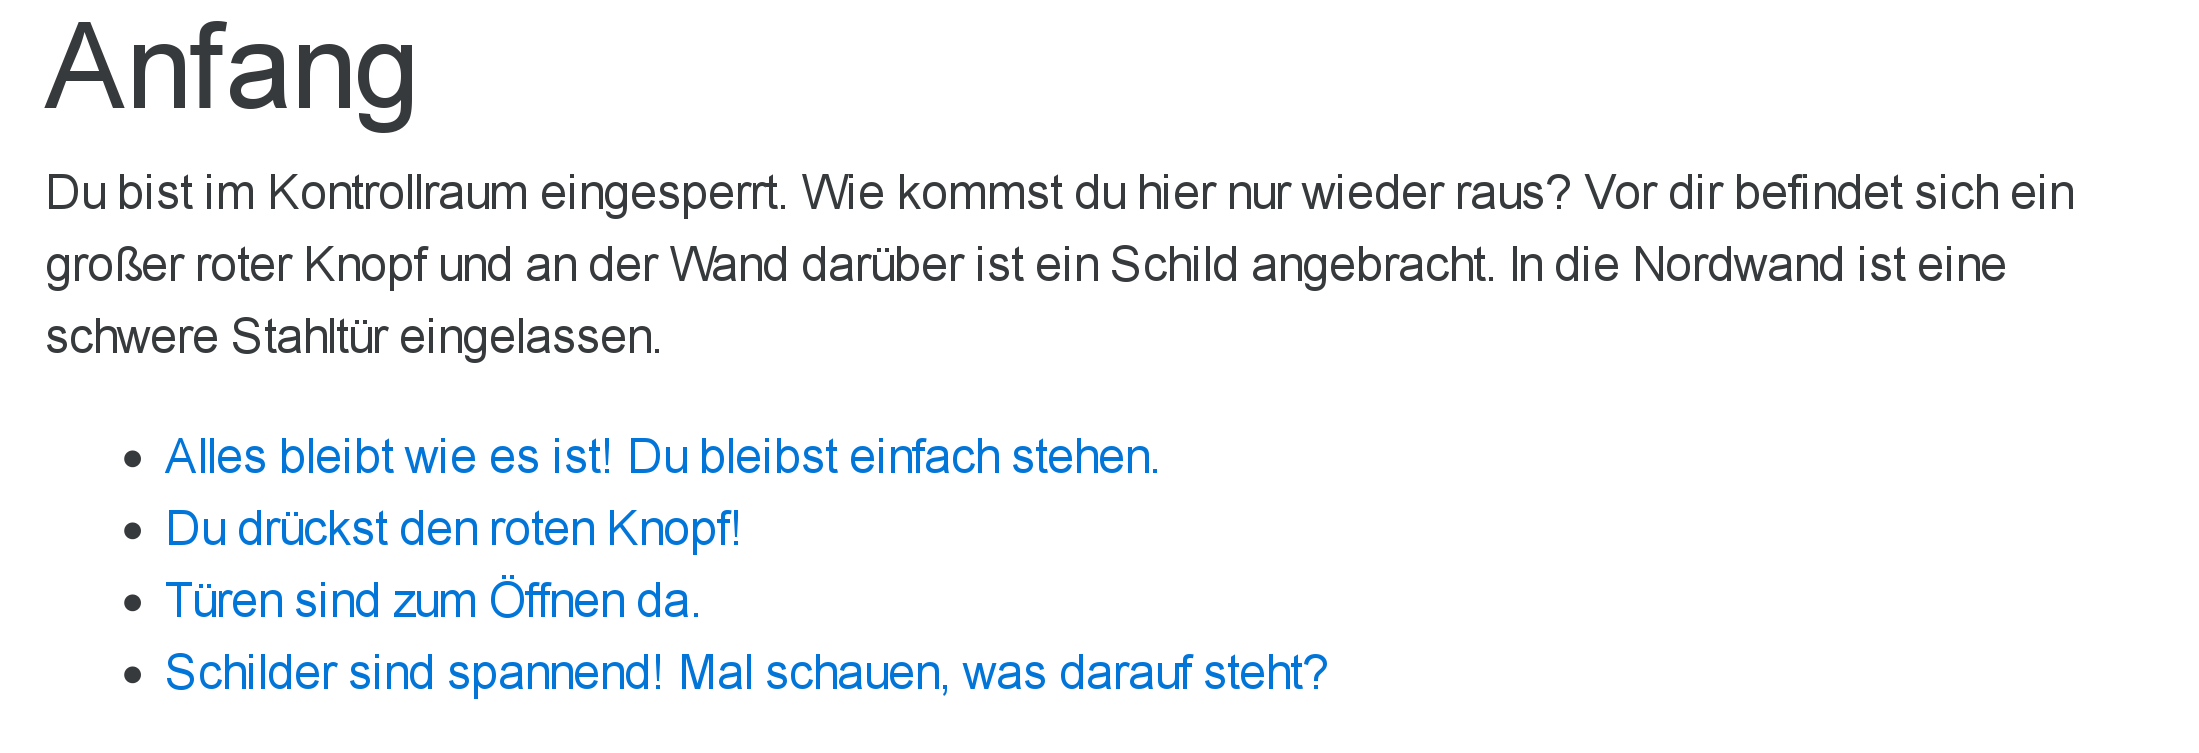
\includegraphics[width=\textwidth-2pt,frame]{images/screenshots/20161019/enduser-cyoa-choice.png}
  \caption{Auswahlmöglichkeiten bei einer interaktiven Geschichte}
  \label{fig:enduser-cyoa-choice}
\end{figure}

Das Datenmodell (siehe Abbildung~\ref{fig:project-cyoa-schema}) für diese Geschichten besteht aus zwei Tabellen: \texttt{chapter} enthält die eigentliche Geschichte, also die Überschrift und den Rumpf aus Abbildung~\ref{fig:enduser-cyoa-choice}. Die Entscheidungsmöglichkeiten werden in \texttt{next\_chapter} hinterlegt. Diese Tabelle stellt eine \texttt{m:n} Beziehungen zwischen Kapiteln her und reichert diese mit einem Entscheidungstext an.

\begin{figure}[h]
  \centering \includegraphics[width=0.8\textwidth]{images/db-schema/cyoa}
  \caption{Schema für interaktive Geschichten}
  \label{fig:project-cyoa-schema}
\end{figure}

Die in Abbildung~\ref{fig:enduser-cyoa-choice} zu sehende Kapitelseite benötigt drei Datenquellen: Per \texttt{GET}-Parameter wird das anzuzeigende Kapitel definiert. Die Abfragen \texttt{kapitel\_einzeln} und \texttt{kapitel\_optionen} benötigen eben jene Kapitel-ID als Parameter und liefern dann den Text des Kapitels selbst sowie die ausgehenden Verweise auf andere Kapitel. Zur Darstellung der Optionen muss aktuell noch auf eine \texttt{HTML}-Einbettung zurückgegriffen werden, Abbildung~\ref{fig:project-cyoa-page-chapter} zeigt den Quelltext innerhalb von \idename{}.

\begin{figure}[h]
  \centering 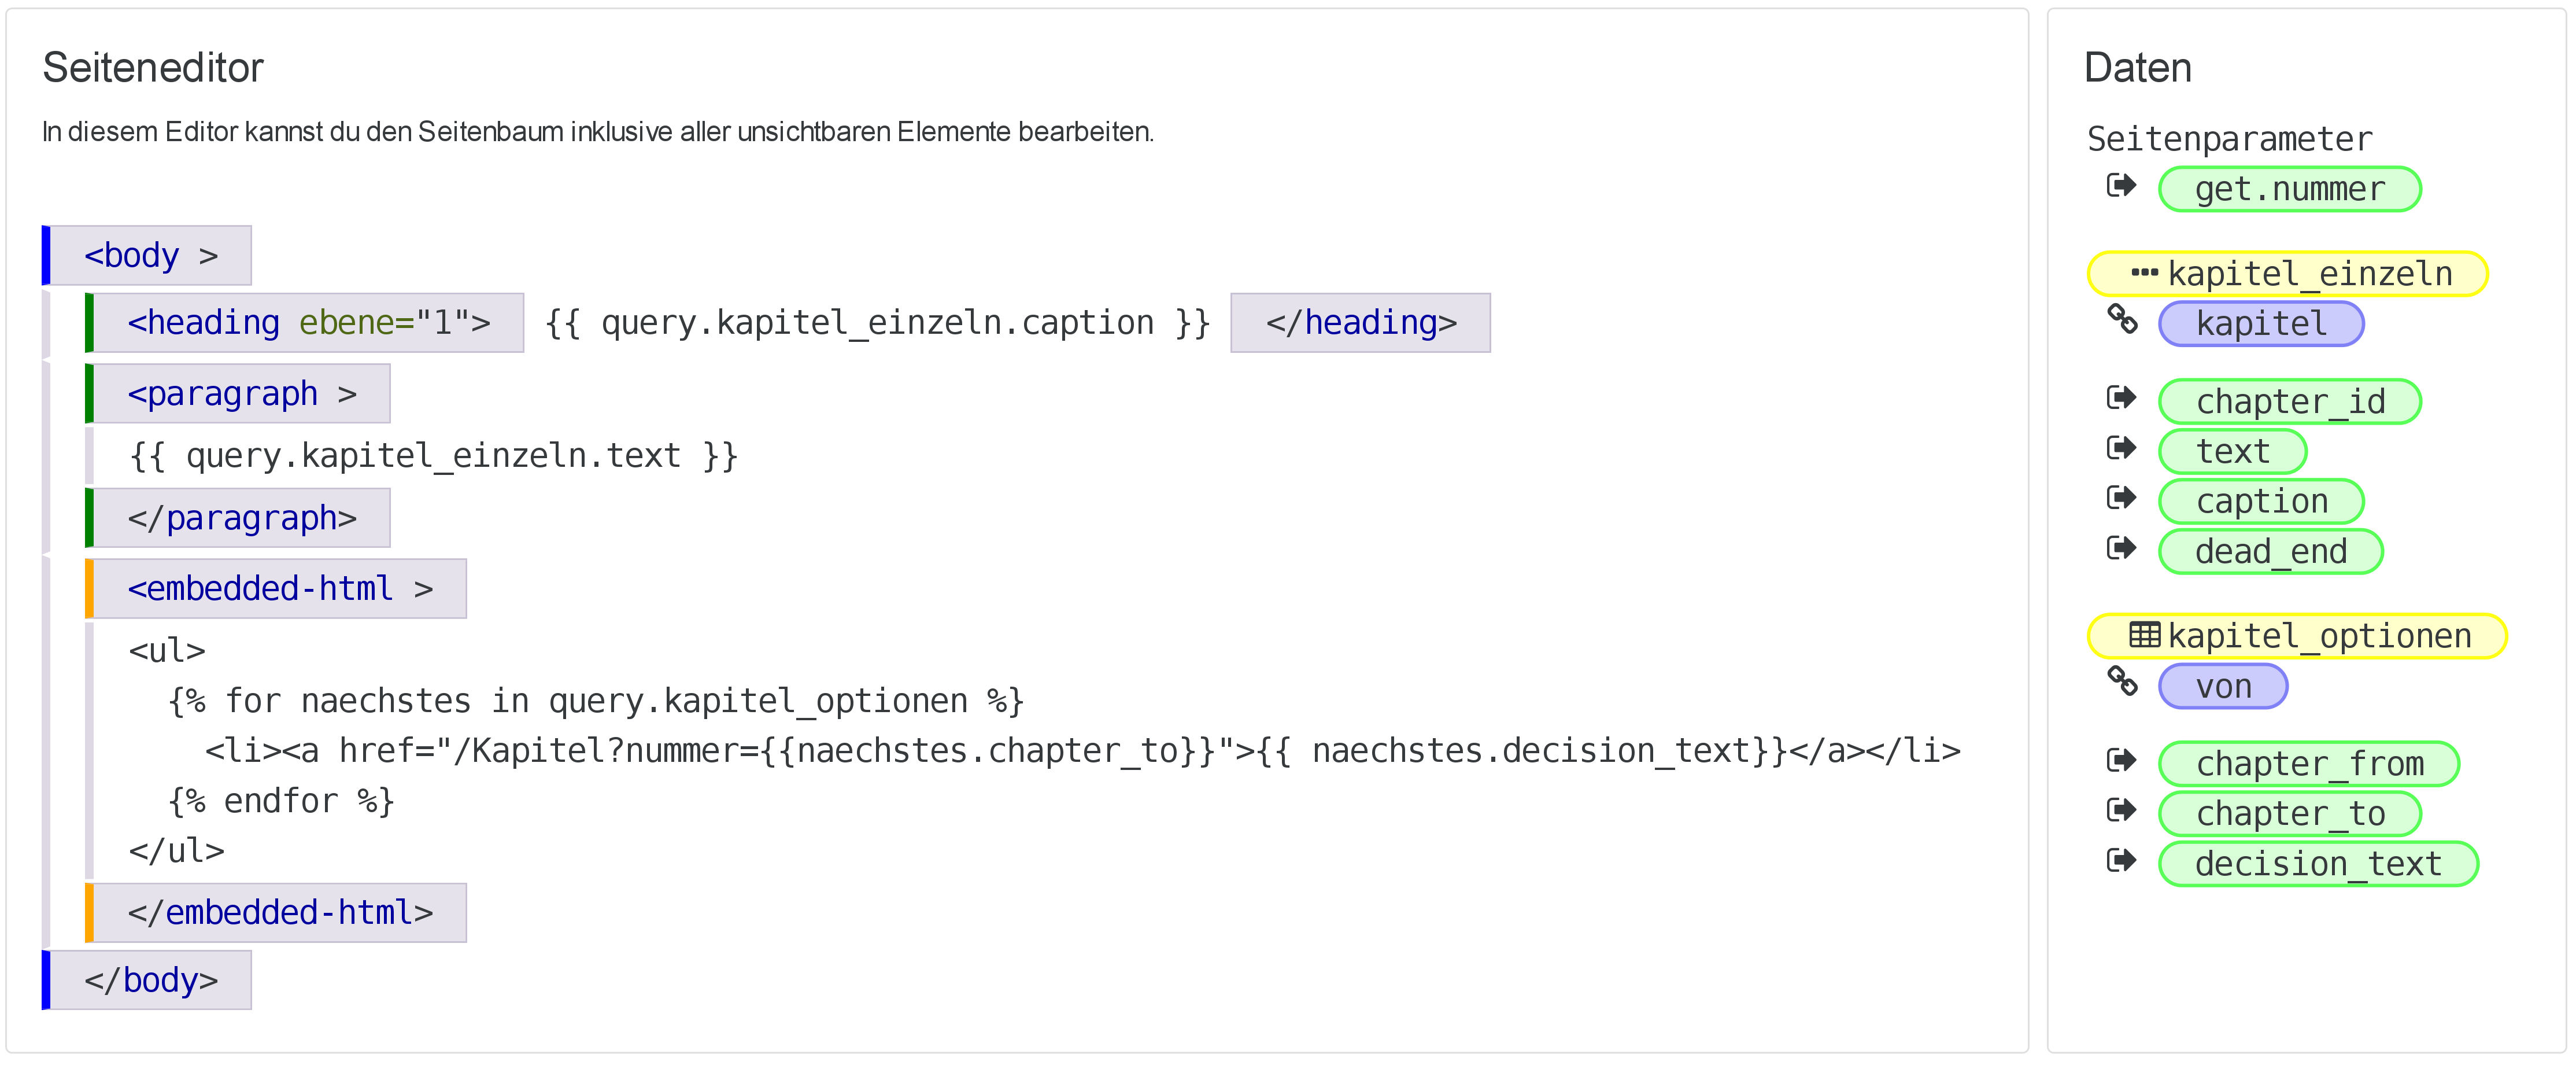
\includegraphics[width=\textwidth]{images/screenshots/20161019/editor-project-cyoa-page-chapter.png}
  \caption{Quelltext für die Anzeige eines Kapitels}
  \label{fig:project-cyoa-page-chapter}
\end{figure}

\subsection{Einfacher Blog mit Kommentaren}

Dieses Beispiel erlaubt die Veröffentlichung von Artikeln durch einen Autor und gibt jedem Leser die Möglichkeit einen Kommentar zu hinterlassen (Abbildung~\ref{fig:enduser-blog-article}), es lässt sich unter \href{http://blog.blattzeug.de/}{blog.blattzeug.de} interaktiv ausprobieren.

\begin{figure}[h]
  \centering \includegraphics[width=\textwidth-2pt,frame]{images/screenshots/20161019/enduser-blog-article.png}
  \caption{Ein (sehr kurzer) Blog-Artikel mit zwei Kommentaren}
  \label{fig:enduser-blog-article}
\end{figure}

Das Datenmodell speichert die eigentlichen Blogbeiträge in der Tabelle \texttt{article}, die dazugehörigen Kommentare in der Tabelle \texttt{comment}. Letztere Tabelle kann von einem normalen Endbenutzer mit weiteren Inhalten gefüllt werden.

\begin{figure}[h]
  \centering 
\includegraphics[width=0.8\textwidth]{images/db-schema/blog}
  \caption{Schema für einen sehr einfachen Blog}
  \label{fig:project-blog-schema}
\end{figure}

Die Seite zur Darstellung eines Blog-Artikels kommt mit den von \idename{} zur Verfügung gestellten Bedienelementen aus. Der anzuzeigende Artikel wird über einen \texttt{GET}-Parameter bestimmt, welcher als Parameter für die Abfragen \texttt{artikel\_detail} und \texttt{artikel\_kommentare} verwendet wird.

Um einen neuen Kommentar zu hinterlassen muss der Endbenutzer in dem Formular seinen Namen und eine Nachricht hinterlassen. Der Knopf "`Kommentieren"' ist mit einer mutierenden Abfrage verknüpft, welche diese Daten dann in der Datenbank hinterlegt.

Anders als die im vorigen Kapitel \fullref{sec:project-cyoa} vorgestellte Seite ist für den Blog kein Einsatz von eingebettetem Quelltext notwendig. Für die Anzeige der Kommentare (siehe Abbildung~\ref{fig:project-blog-page-article}) wird die eingebaute Datentabelle herangezogen, allerdings nur mit einer Teilmenge der verfügbaren Spalten. Schließlich spielt die \texttt{ID} des Artikels oder Kommentars in der Darstellung für Endanwender keine Rolle.

\begin{figure}[h]
  \centering 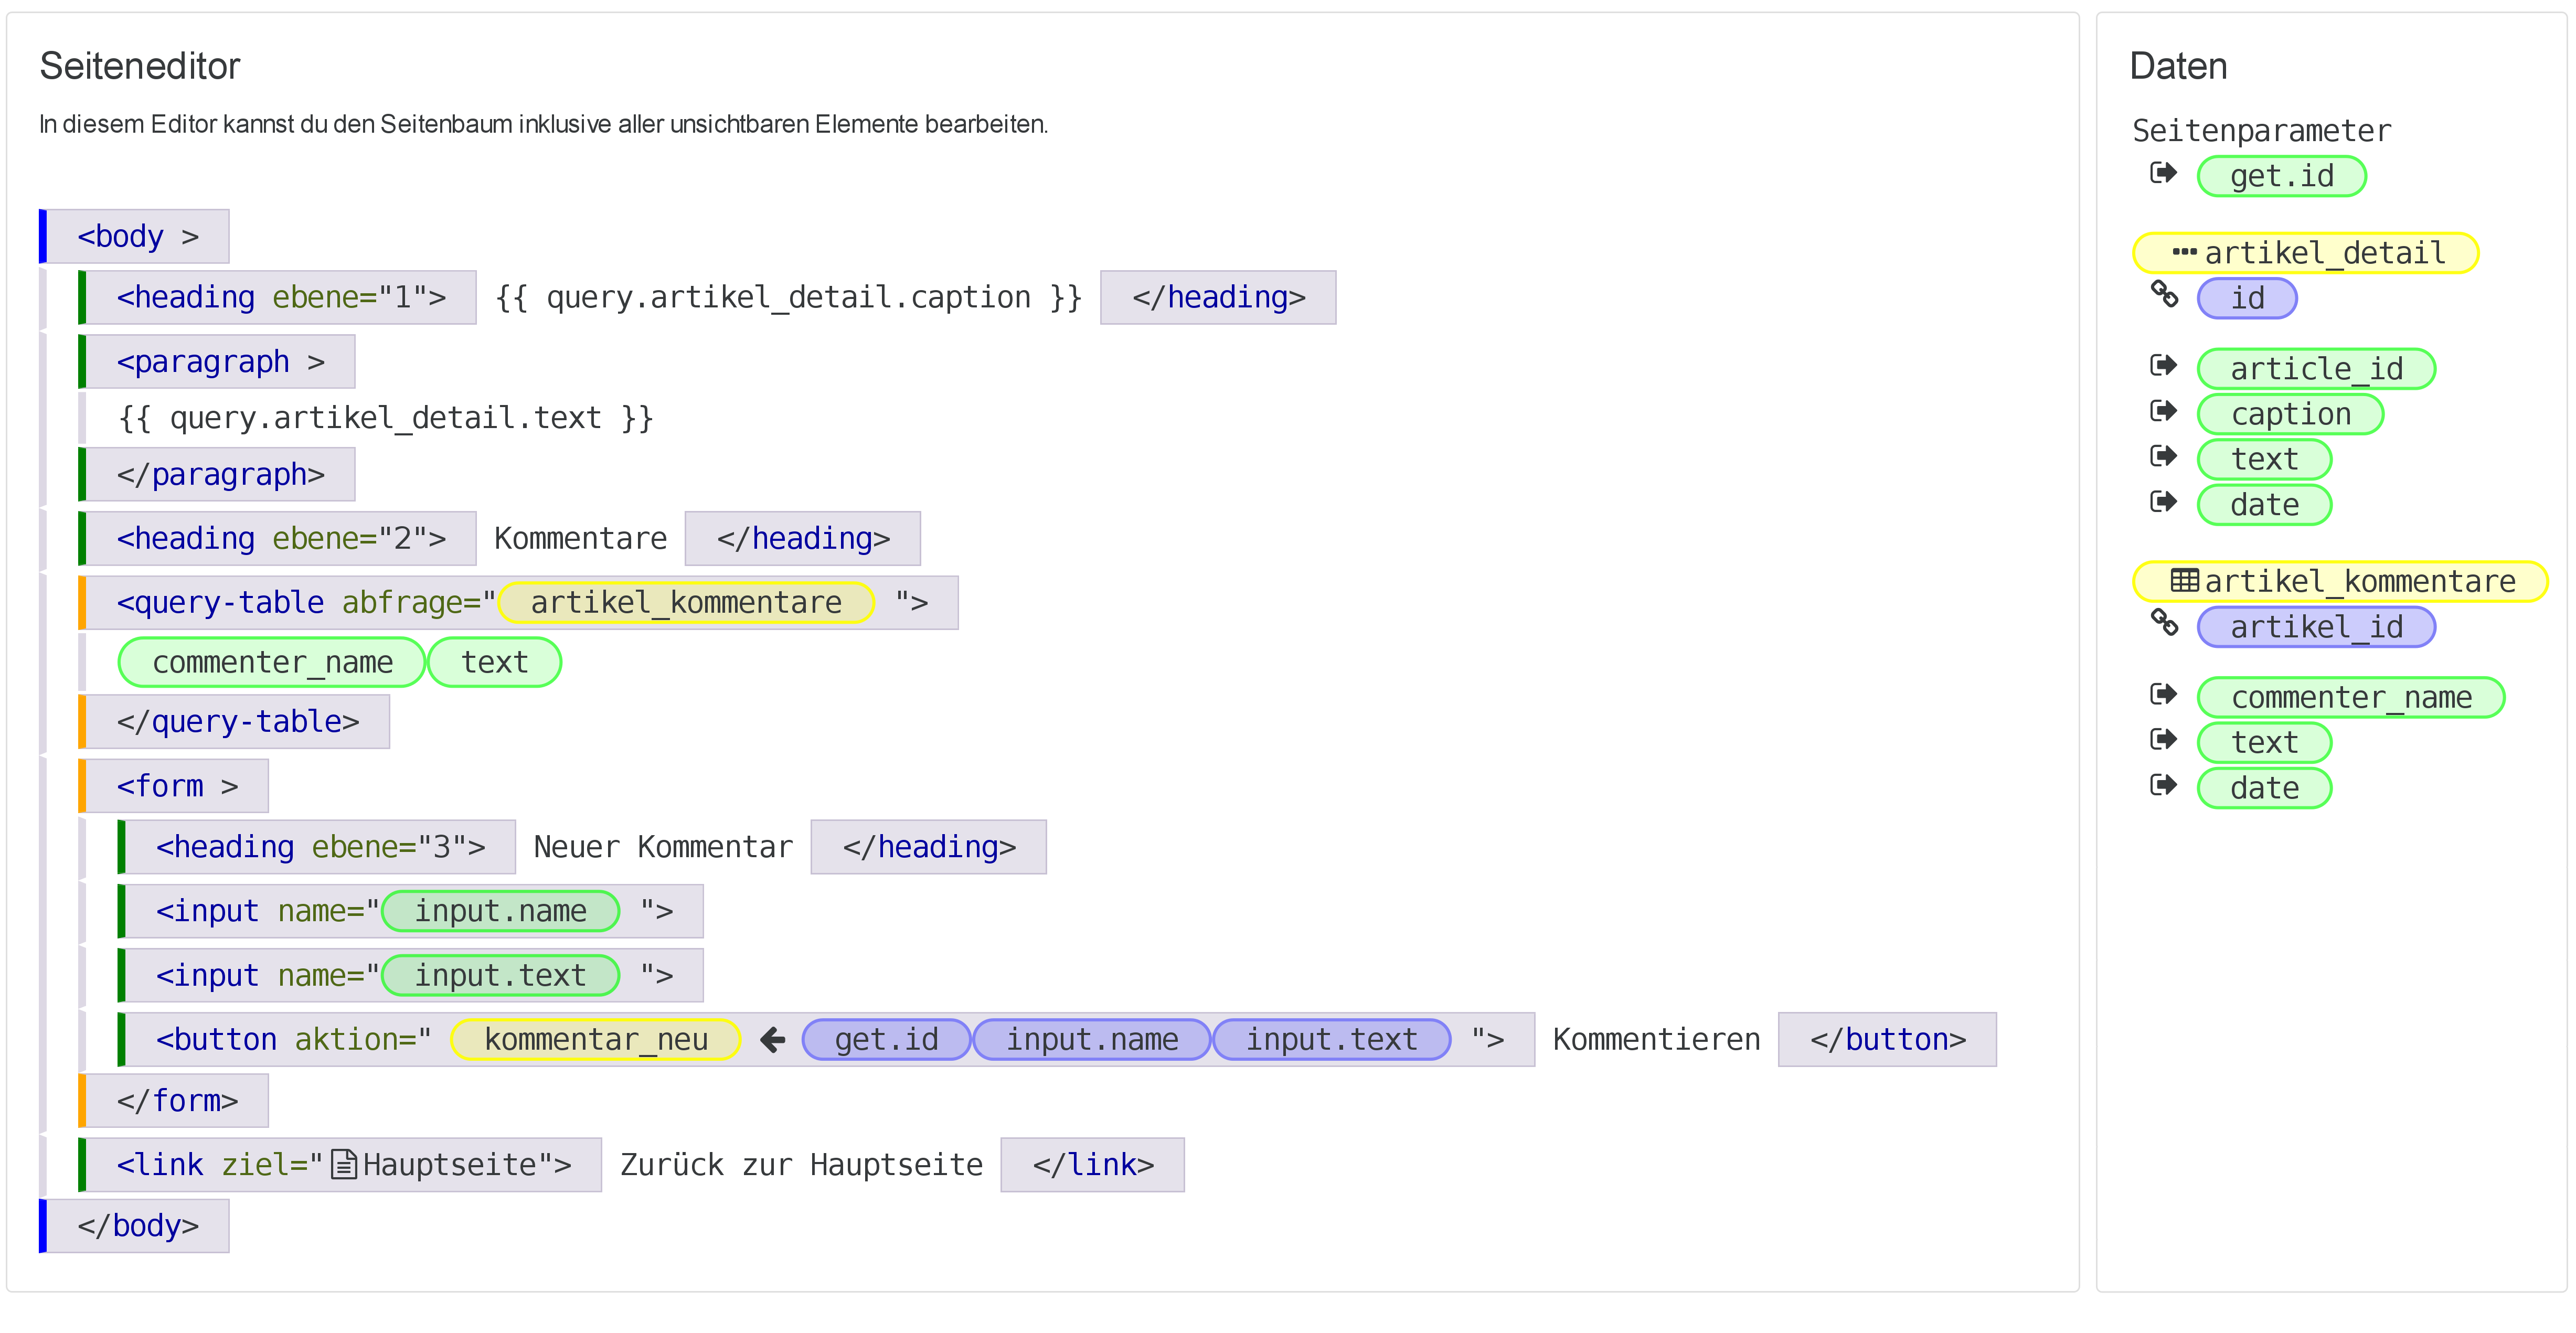
\includegraphics[width=\textwidth]{images/screenshots/20161019/editor-project-blog-page-article.png}
  \caption{Quelltext für die Anzeige eines Blog-Artikels}
  \label{fig:project-blog-page-article}
\end{figure}

\subsection{Pokémon Go}

Dieses Projekt fungiert als eine virtuelle Vitrine um die eigenen Spielfiguren aus Pokémon Go auszustellen. Der hinter dem Spiel stehende Datenbestand eignet sich prinzipiell gut zur Erläuterung von Problemen bei redundanten Daten, der aktuell implementierte Stand gibt diesen Schwerpunkt aber noch nicht sehr gut wieder. Die ausgestellten Pokémon lassen sich von Endbenutzern sowohl anlegen als auch löschen (siehe Abbildung~\ref{fig:enduser-pokemongo-delete}), was unter \href{http://pokemongo.blattzeug.de/}{\mbox{pokemongo.blattzeug.de}} ausprobiert werden kann.

\begin{figure}[h]
  \centering 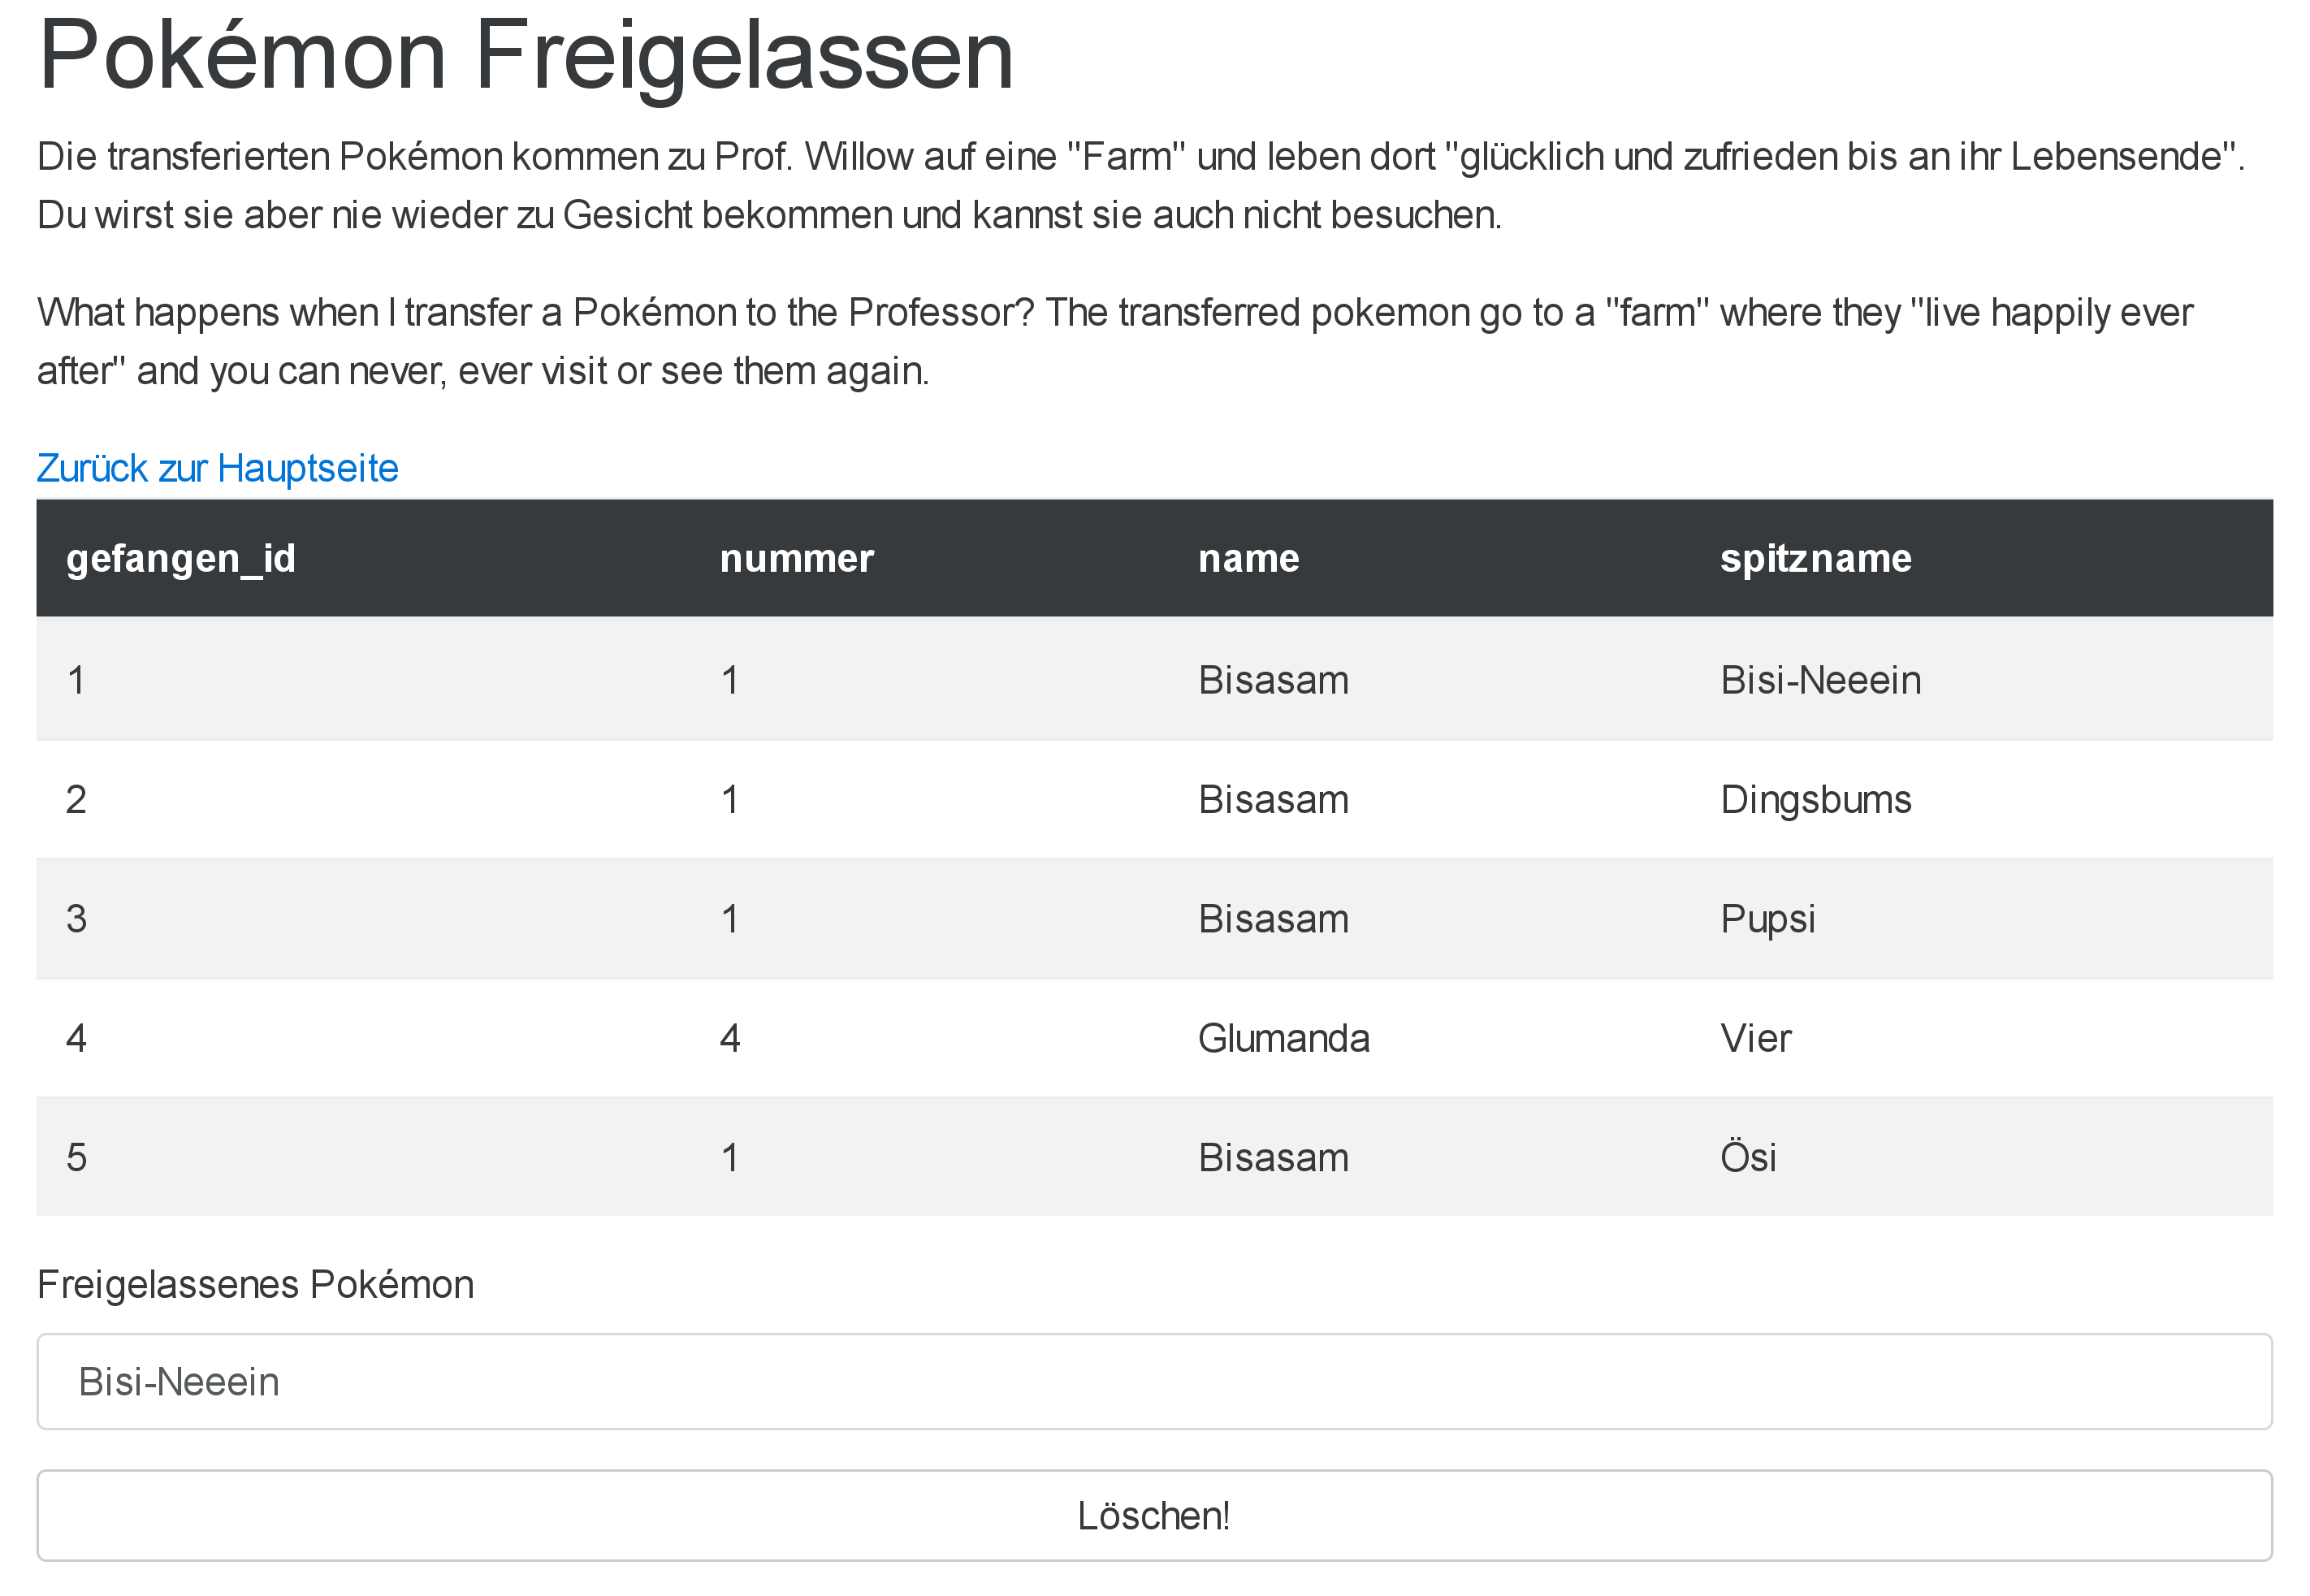
\includegraphics[width=\textwidth-2pt,frame]{images/screenshots/20161019/enduser-pokemongo-free.png}
  \caption{Löschen eines gefangenen Pokémon}
  \label{fig:enduser-pokemongo-delete}
\end{figure}

Das aktuell implementierte Schema des Beispiels besteht aus zwei Tabellen. Die Bezeichnung "`Pokémon"' wurde dabei vermieden, da sich eine komplette Spielfigur nur aus mehreren Tabellen zusammenstellen lässt. Die Tabelle \texttt{pokedex} enthält dabei gewissermaßen die Stammdaten der Spielfigur: Dabei handelt es sich um den übergeordneten Namen und einen Typ. Da ein Spieler jedes Pokémon auch mehrfach besitzen kann sind diese Daten als unveränderlich anzusehen. Die konkreten Pokémon eines Spielers ergeben sich dann aus der Tabelle \texttt{gefangen}. Hier sind die Variablen Werte einer Spielfigur, also der frei wählbare Spitzname und die im Spiel verfügbare Stärke, hinterlegt.

An Abbildung~\ref{fig:enduser-pokemongo-delete} lässt sich erkennen, mit welcher Art Daten diese Tabellen gefüllt sind: Der Inhaber der Seite hat mehrere Varianten des Pokémon "`Bisasam"' gefangen, diese haben unterschiedliche Spitznamen bekommen und sind unterschiedlich stark.

Inhaltlich weist diese Schema noch einige Verletzungen von gutem Datenbankdesign auf: Der Typ eines Pokémon ist nicht wahlfrei, sondern eine feste Aufzählung aus Werten wie "`Feuer"', "`Wasser"', ... Ferner kann jedes Pokémon inhaltlich nicht nur einen, sondern zwei Typen haben. An dieser Stelle müsste das Datenmodell also noch angepasst werden.

\begin{figure}[h]
  \centering \includegraphics[width=0.8\textwidth]{images/db-schema/pokemongo}
  \caption{Schema für Pokémon Go}
  \label{fig:project-pokemongo-schema}
\end{figure}

Aus Sicht eines Entwicklers ist an dem "`Pokémon Freilassen"'-Bilschirm vor allem interessant, dass die Abfrage zur Auflistung aller eigenen (\texttt{Meine\_Pokemon}) Pokémon von zwei Bedienelementen verwendet wird (Abbildung~\ref{fig:project-pokemongo-page-delete}). Sowohl die Datentabelle zur Anzeige der eigenen Fänge als auch die Auswahl des zu löschenden Datensatzes in dem Formular machen davon Gebrauch.

\begin{figure}[h]
  \centering \includegraphics[width=0.95\textwidth]{images/screenshots/20161019/editor-project-pokemongo-page-delete.png}
  \caption{Quelltext der Seite zum Löschen eines gefangenen Pokémon}
  \label{fig:project-pokemongo-page-delete}
\end{figure}

%%% Local Variables:
%%% mode: latex
%%% TeX-master: "thesis"
%%% End:
